\documentclass[a4paper,12pt,fleqn,oneside]{article}
\usepackage{etex}
\usepackage[utf8]{inputenc}
\usepackage{ae,aecompl}
\usepackage[T1]{fontenc}
\usepackage{ngerman}
\usepackage{fleqn}
\usepackage{ulem}
\usepackage{amssymb}
\usepackage{tabularx}
\usepackage{bm}
\usepackage{color}
\usepackage{pictex}
\usepackage[left=2.5cm,right=2.5cm,top=2cm,bottom=2cm,includeheadfoot]{geometry}
\usepackage[section]{placeins}
\usepackage{xspace}
\usepackage{multirow}
\usepackage{lastpage}
\usepackage{fancyhdr}
\usepackage{graphicx}
\usepackage{esvect}
\usepackage{textcomp}
\usepackage{amssymb}
\usepackage{fixltx2e }
\usepackage{graphicx}
\setlength{\headheight}{15pt}
\pagestyle{fancy}
\fancyfoot[C]{Seite \thepage{} von \pageref{LastPage}}
\linespread{1.5}
\author{Dominik Eisele}
\title{Dokumentation zur GFS "`Digitales Rechenwerk"'}
\date{\today}

\Huge

\newcolumntype{L}[1]{>{\raggedright\arraybackslash}p{#1}}
\newcolumntype{C}[1]{>{\centering\arraybackslash}p{#1}}
\newcolumntype{R}[1]{>{\raggedleft\arraybackslash}p{#1}}


\setlength{\tabcolsep}{0pt}
\renewcommand{\arraystretch}{1}

\renewcommand*\contentsname{Gliederung}

\let\oldsqrt\sqrt
\def\sqrt{\mathpalette\DHLhksqrt}
\def\DHLhksqrt#1#2{\setbox0=\hbox{$#1\oldsqrt{#2\,}$}\dimen0=\ht0
\advance\dimen0-0.3\ht0
\setbox2=\hbox{\vrule height\ht0 depth -\dimen0}
{\box0\lower0.4pt\box2}}

\begin{document}


\normalem

\begin{titlepage}
	\maketitle
\end{titlepage}

	\tableofcontents

\newpage


	\section{Rechnen mit dualen Zahlen}
	\subsection{Addition von Dualzahlen}
		Die Addition von Dualzahlen verläuft im Prinzip wie die Addition von Dezimalzahlen, sobald die Addition an einem
		Stellenwert den maximalen Stellenwert übersteigt erfolgt ein Übertrag auf die nächste Stelle.\\
		Rechenregeln:
		\[ \begin{array}{rcll}
   				 0 + 0 & = & 0													\\
  			         0 + 1 & = & 1													\\
    				 1 + 1 & = & 0$ (+ 1 Übertrag)$										\\
    			   1 + 1 + 1 & = & 1$ (+ 1 Übertrag)$
		\end{array} \]
		Beispiel:
		\[ \begin{array}{lrcll}
   					&		 	       	 1 1 1 0 1 0 0 1 0 		 	 & = & 466 		\\
  			       	$+ $ &				 0 0 1 1 1 0 1 0 0			 & = & 116		\\
  			       	$Ü $ &      			      1 1 1 1 1 1$ $$ $$ $$ $$ $$ $         				\\
    					&	\_\_\_\_\_\_\_\_\_\_\_\_\_\_\_\_\_\_							\\
    			   		&			      1 0 0 1 0 0 0 1 1 0			 & = & 582
		\end{array} \]

\newpage

	\subsection{Subtraktion von Dualzahlen}
  		Bei der Subtraktion von Dualzahlen gelten die gleichen Rechenregeln, wie bei der Subtraktion von Dezimalzahlen.\\
  		Rechenregeln:
		\[ \begin{array}{rcll}
   			 0 - 0 & = & 0													\\
  		         0 - 1 & = & 1$ (+ 1 Entlehnung)$									\\
    			 1 - 0 & = & 1													\\
			 1 - 1 & = & 0													\\
    		    0 - 1 - 1 & = & 0$ (+ 1 Entlehnung)$									\\
    		    1 - 1 - 1 & = & 1$ (+ 1 Entlehnung)$
		\end{array} \]
		Beispiel:
		\[ \begin{array}{lrcll}
   				&		 	       	 1 1 1 0 1 0 0 1 0 		& = & 466 			\\
  		       	$- $ &				 0 0 1 1 1 0 1 0 0 		& = & 116				\\
  		       	$E $ &      			            1 1 1 1 1$ $$ $$ $$ $        	 				\\
    				&	\_\_\_\_\_\_\_\_\_\_\_\_\_\_\_\_\_\_							\\
    		   		&			      	  1 0 1 0 1 1 1 1 0		 & = & 350
		\end{array} \]

\newpage

	\subsection{Subtraktion mit dem Zweierkomplement}
		Da, in der Digitaltechnik, für die Subtraktion von Dualzahlen keine logische Verknüpfung existiert, ist man gezwungen eine
		Subtraktion in eine Addition umwandeln.
		\[ \begin{array}{rcl}
   				 2 - 6       & = & (-4)			\\
  			         2 + (-6)   & = & (-4)
		\end{array} \]
		\vspace{\baselineskip}
		Diese Umwandlung geschieht mit Hilfe des Zweierkomplements. Es wird gebildete in dem man den Subtrahend auf die volle
		Stellenzahl erweitert (Nullen nach links auffüllen). Hierbei muss die Breite der Komplementdarstellung beider Zahlen
		berücksichtigt werden. Üblich sind 4, 8, 16, 32 und 64 Bit. Als nächstes muss der Subtrahend negiert werden, das heißt
		man lässt jedes einzelne Bit kippen. Zu dem gebildeten bitweisen Komplement muss $+ 1$ hinzuaddiert werden. Das nun
		erhaltene Zweierkomplement muss man mit dem Minuenden addieren um das Zweierkomplement-Ergebnis der eigentlichen
		Subtraktion zu erhalten. Um das nun eigentliche Ergebnis zu erhalten muss man das Ergebnis negieren und wieder $+ 1$
		addieren. Das höchstwertigste Bit des Zweierkomplement-Ergebnisses, stellt dabei das Vorzeichen da, und wird nicht zur
		Negation verwendet. Wenn es eine 1 ist, ist das Endergebnis negativ, bei einer 0 ist es positiv. \\
		\\

\newpage

		Beispiel:\\
		$ 2 - 6 =$ $ ? $ \\
		\\
		1. Schritt: In eine Dualzahl wandeln:\\
		$ 2 - 6 \Rightarrow 10 - 110$\\
		\\
		2. Schritt: Stellen auffüllen:\\
		$ 0010 - 0110 =$ $ ? $\\
		\\
		3. Schritt: Bits negieren:\\
		$ 0110 \Rightarrow 1001$\\
		\\
		4. Schritt: Hinzuaddieren von 1:\\
		$ 1001 + 0001 = 1010$\\
		\\
		5. Schritt: Minuend und Zweierkomplement addieren:\\
		$ 0010 + 1010 = 1100$\\
		\\
		6. Schritt: Ergebnis negieren:\\
		$ 100 \Rightarrow 011$\\
		\\
		7. Schritt: Hinzuaddieren von 1:\\
		$ 011 + 001 = 100$\\
		\\
		8. Schritt: In eine Dezimalzahl wandeln:\\
		$ 100 \Rightarrow 4$ ; da das höchstwertige Bit 1 ist: Endergebnis $=$ $ -4$\\

\newpage

	\subsection{Multiplikation von Dualzahlen}
		Auch die binäre Multiplikation wird nach denselben Regeln durchgeführt, wie die dezimale Multiplikation. Dabei werden
		Produkte mit den einzelnen Stellen des Multiplikators gebildet und anschließend Stellenrichtig addiert. Gegenüber der
		dezimalen Multiplikation bringt die binäre Multiplikation Vereinfachungen mit sich. Da die Stellen des Multiplikators nur die
		Zahlenwerte Null und Eins annehmen können, muss der Multiplikand nur mit Null und Eins multipliziert werden. Bei der
		binären Multiplikaton kommen als Teiloperationen nur die Addition und Verschiebung vor.\\

		Beispiel:
			\[ \begin{array}{lrcll}
   					&		 	       	\uline{1 0 1 1 \times 1 0 1 0}   	 				\\
  			       		&   			            1 0 1 1 $ $$ $$ $$ $$ $$ $        	 			\\
					&   			            0 0 0 0 $ $$ $$ $$ $        	 				\\
					&   			            1 0 1 1 $ $$ $        	 					\\
				$+ $	&   			            0 0 0 0			        	 				\\
					&	\_\_\_\_\_\_\_\_\_\_\_\_\_\_\_						\\
					&				    1101110
			\end{array} \]



\newpage

	\section{Umsetzung in eine Digitale Rechenschaltung}
	\subsection{Addierer}
		\subsubsection{Halbaddierer}
		Ein Halbaddierer besitzt zwei Ein-, und zwei Ausgänge. An die Eingänge \emph{x} und \emph{y} werden jeweils die Ziffern
		angelegt die man addieren möchte. An dem ersten Ausgang liegt die Summe $s$ der Addition an, am zweiten Ausgang der 
		Übertrag $c$.\\
		Daraus ergibt sich die Wertetabelle \ref{tab:halbaddierer}.
		\begin{table}[h]
			\center
			\begin{tabular}{c|c|c|c}
				\ \textbf{x} \ 	& \ \textbf{y} \ 	& \ \textbf{Übertrag c} \ & \ \textbf{Summe s} \ 	 	\\ \hline
				0 	& 0 		& 0          		& 0       			\\ \hline
				0 	& 1 		& 0          		& 1       			\\ \hline
				1 	& 0		& 0          		& 1      			 \\ \hline
				1	& 1 		& 1          		& 0      			 \\
			\end{tabular}
			\caption{Wertetabelle Halbddierer}
			\label{tab:halbaddierer}
		\end{table}

		\noindent
		In Schaltungen wird der Halbaddierer aus zwei Bauteilen zusammengesetzt, ein Exklusiv-ODER (XOR) und ein UND (AND).\\
		Der Aufbau des Halbaddierers ist in Abbildung \ref{fig:halbaddierer} dargestellt.

		\begin{figure}[h]
			\center
			\input skizze_halbaddierer
			\caption{Halbaddierer}
			\label{fig:halbaddierer}
		\end{figure}


\newpage

	\subsubsection{Volladdierer}
		Der Volladdierer besteht aus zwei Halbaddierern und einem ODER. Da ein Volladdierer einen zusätzlichen Eingang
		(c\textsubscript{in}) hat, kann man mit ihm den Übertrag aus einer vohergegangenen Addition mit in die Rechnung
		einbeziehen. Man kann somit mehrere Volladdierer hintereinander schalten um größere Zahlen miteinander zu addieren.
		Dabei verbindet man den Carry out Ausgang mit dem Carry in Ausgang des höherwertigen Volladierers.\\
		Daraus ergibt sich die Wertetabelle \ref{tab:volladdierer}.



		\begin{table}[h]
			\center
			\begin{tabular}{c|c|c|c|c}
			\textbf{ \ x \ } & \textbf{ \ y \ } & \textbf{ \ c\textsubscript{in} \ } & \textbf{ \ c\textsubscript{out} \ } & 
														\multicolumn{1}{l} {\textbf \ {s \ }} \\ \hline
			0          & 0          & 0            & 0             & 0                              \\ \hline
			0          & 0          & 1            & 0             & 1                              \\ \hline
			0          & 1          & 0            & 0             & 1                              \\ \hline
			0          & 1          & 1            & 1             & 0                              \\ \hline
			1          & 0          & 0            & 0             & 1                              \\ \hline
			1          & 0          & 1            & 1             & 0                              \\ \hline
			1          & 1          & 0            & 1             & 0                              \\ \hline
			1          & 1          & 1            & 1             & 1
			\end{tabular}
			\caption{Wertetabelle Volladdierer}
			\label{tab:volladdierer}
		\end{table}

		\noindent
		In Schaltungen wird der Volladdierer aus zwei Halbaddierern und einem ODER (OR) zusammengesetzt.\\
		Der Aufbau des Halbaddierers ist in Abbildung \ref{fig:volladdierer} dargestellt.

		\begin{figure}[h]
			\center
			\input skizze_volladdierer
			\caption{Volladdierer}
			\label{fig:volladdierer}
		\end{figure}

\newpage

	\subsection{Subtrahierer}
		Beim Subtrahierer wird der Volladdierer durch einen Steuereingang erweitert. An diesem legt man für eine Addition eine
		$0$, und für eine Subtraktion eine $1$ an. Diesen Steuereingang legt man, zusammen mit dem y-Eingang, an ein
		Exklusiv-ODER (XOR). Der Ausgang dieses Exklusiv-ODERs wird an den ursprünglichen $y$ Eingang angelegt. Somit wird
		der $y$ Wert, bei einer am Steuereingang anliegenden logischen $1$ negiert. Bei dem niederwertigsten Subtrahierer muss
		zudem das Steuersignal auf den Carry in Eingang gelegt werden um die, für die Zweierkomplementrechnung benötigte, 1
		zu addieren. Zu sehen ist dieser Aufbau in Abbildung \ref{fig:steuerbarer_volladdierer}.

		\begin{figure}[h]
			\center
			\input skizze_volladdierer_steuerbar
			\caption{Volladdierer mit Steuerleitung zum Subtrahieren}
			\label{fig:steuerbarer_volladdierer}
		\end{figure}



\newpage

	\subsection{Rechenwerk}
		Das in Abbildung \ref{fig:Addierwerk} gezeigte Schaltnetz besteht aus acht kaskadierten Volladdierern. Zusätzlich besitzen
		sie jeweils einen Steuereingang, mit welchem der Summand, der aus den $y$ Bestandteilen aufgebaut ist, negiert werden
		kann, sodass mit Schaltnetz auch Subtraktionen durchgeführt werden können.\\
		Um eine Rechenoperation durchzuführen muss man die Summanden $x$ und $y$ an die Eingänge $x_1$ bis $x_n$ und
		$y_1$ bis $y_n$ anlegen. An die Steuereingänge legt man eine logische $0$ für eine Addition, und eine logische $1$ für
		eine Subtraktion an. Die Endsumme liegt an den Ausgängen $z_1$ bis $z_n$ an.


		\begin{figure}[h]
			\center
			\input skizze_addierwerk
			\caption{Steuerbares Addierwerk}
			\label{fig:Addierwerk}
		\end{figure}
	\FloatBarrier



\newpage

	\subsection{Multiplizierer}
		Der in Abbildung \ref{fig:Multiplizierer} gezeigte Multiplizierer kann zwei acht Bit Zahlen miteinander multiplizieren. Dazu 
		legt man seine erste Zahl ($2.1 - 2.8$) an ein Schieberegister an, sodass die Zahl bei jedem Takt um eine Stelle verschoben 
		werden kann. Dann wird pro Takt die höchstwertigste Ziffer des Multiplikators abgegriffen, die anschließend mit dem 
		Multiplikant multipliziert wird. Da die abgegriffene Ziffer nur die Zustände  "`Null"' und  "`Eins"' annehmen kann, kann man 
		die Multiplikation mit einfachen UND-Verknüpfungen realisieren. Um die Produkte auch Stellenrichtig addieren zu können 
		muss man die Zwischenergebnisse ebenfalls pro Takt verschieben. Dies wird gelößt indem man ein Register nimmt, 
		welches das Ergebniss um eine Stelle versetzt wieder auf den Addierer gibt. Der selben Aufbau aus Register und Addierer 
		wird auch verwendet um die, aus dem ersten Addierer hinausgeschobenen, Stellen aufzufangen. Das Produkt kann man, 
		nach acht Takten Rechenzeit, an den Ausgängen der Addierer abgreifen. Da die Steuereinheit aus Abbildung 
		\ref{fig:Steuereinheit_Multiplizierer} das Taktsignal einen Takt zu spät stoppt, muss man das Ergebnis durch zwei teilen, 
		indem man die Ziffern des Produktes jeweils an dem nächst höherwertigen Pin abgreift.\\
		 
		
		\begin{figure}[h]
			\center
			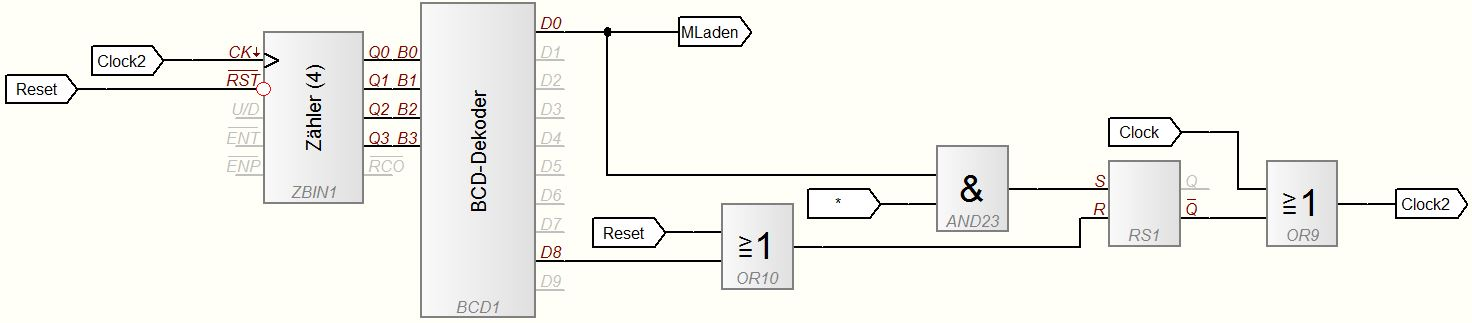
\includegraphics[width=0.7\textwidth]{steuereinheit_multiplizierer}
			\caption{Steuereinheit 8-Bit Multiplizierer}
			\label{fig:Steuereinheit_Multiplizierer}
		\end{figure}

		Die in Abbildung \ref{fig:Steuereinheit_Multiplizierer} sichtbare Steuereinheit des 8-Bit Multiplizierers ist dafür 
		verantwortlich, dass der Takt "`ClMult"' am Anfang er Rechenoperation gestartet, und nach acht Takten wieder gestoppt 
		wird. Wenn D\textsubscript{0} nach einem Reset $1$ ist, wird das ladbare Schieberegister geladen. Ist zusätzlich dazu 
		noch der Taster "`*"' gedrückt, wird der Ausgang \={Q} des  Flip-Flops  $0$, sodass der Main-Clock auch der Clock des 
		Multiplizierers wird. Acht Takte später, wenn der Ausgang D\textsubscript{8} $1$ ist, wird der Reseteingang des Flip-Flops
		 $1$, sodass \={Q}  wieder 1 ist und der Takt blockiert wird. So wird der Multiplizierer gestoppt, sodass das Produkt 
		abgelesen werden kann. 

		\begin{figure}[h]
			\center
			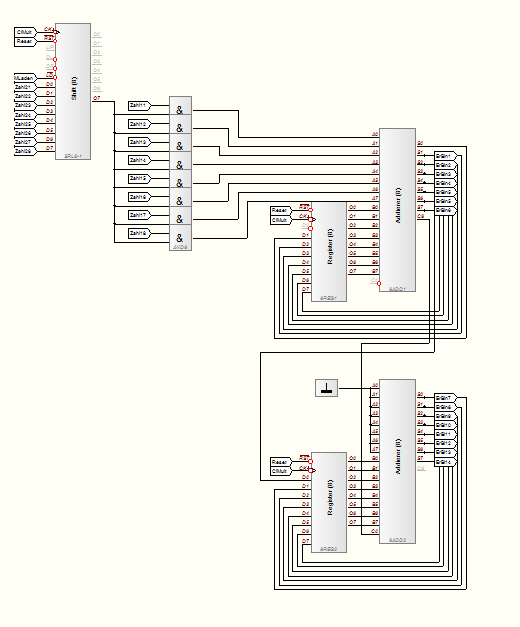
\includegraphics[width=0.7\textwidth]{multiplizierer}
			\caption{8-Bit Multiplizierer}
			\label{fig:Multiplizierer}
		\end{figure}














\end{document}
